% !TEX root = main.tex
%preliminära resultat som kan demonstreras vid halvtidskontroll
\chapter{Results}\label{cha:result}
This section describes the results considering performance, robustness and stability with respect to the different control approaches. The benchmark results of each approach will first be presented individually and then in a comparison in the end.

\section{Benchmark test}
Each of the control approaches have been evaluated with respect to robustness to model errors, disturbance rejection, closed loop bandwidth and response to step, ramp and sinusoidal input summarized below.

\begin{itemize}
\item {\bf Step, ramp and periodical tracking} - A step, ramp and periodic input is applied on the input to benchmark the tracking capability of the controller.
\item {\bf Disturbance rejection} - Modified step responses with added noise is applied to the input to benchmark how sensitive the system is to system disturbances.
\item {\bf Robustness to model errors} - During operation with a periodic input signal, the dynamical model is changed and the output is studied to characterize the robustness to model errors.
\end{itemize}

\section{Simulation Results}
\subsection{Model Reference Adaptive Control}

For the comparison between the adaptive and the present control approach, the adaptive control laws were discretized by using Tustin's formula with a sampling frequency of 2kHz. The high order system model in \eqref{eq:tf} was used to model the rotational stage dynamics. However, a second order model approximating the higher order system was used in the adaptive control laws to keep the computational burden low. The discretized reference model can be seen in \eqref{eq:sys_gm} and all parameters and tuning variables is summerized in Table~\ref{tab:adaptive_param}. The controller is tuned to be robust to input disturbances and model changes. The set of parameter presented in Table~\ref{tab:adaptive_param} is not an optimal set but a decent set of parameters that maintains stability for stepsizes below 20mrad.

\begin{equation}
  \label{eq:sys_gm}
  G_m(z) = \frac{7.9z + 6.7}{1313z^{2} - 2095z + 796.4}
\end{equation}

\begin{table}[h!]
  \centering
  \begin{tabular}{| l | l |}
    \hline
    Parameter & Value \\ \hline
    $T_s$ & $5 \times 10^{-4}$ \\
    $\alpha_0$ & $5.7 \times 10^{4}$ \\
    $\alpha_1$ & $7.2$ \\
    $\beta_0$ & $7.5 \times 10^{7}$ \\
    $a_0$ & $5.7 \times 10^{4}$ \\
    $a_1$ & $1 \times 10^{3}$ \\
    $b_0$ & $7.5 \times 10^{7}$ \\
    $\eta_0$ & $3 \times 10^{-2}$ \\
    $\eta_1$ & $1 \times 10^{-1}$ \\
    $\eta_2$ & $1 \times 10^{-10}$ \\
    $\eta_3$ & $1 \times 10^{-17}$ \\
    $\epsilon$ & $1 \times 10^{-8}$ \\
    $Q$ & $diag(1 \times 10^{10}, 1 \times 10^{-3})$\\
    \hline
  \end{tabular}
  \caption{\label{tab:adaptive_param} Parameters of the system model and the tuned adaptive controller.}
\end{table}

Figure~\ref{fig:step_adaptive} shows the step repsonse to different stepsizes. Here it is clear that the system becomes unstable if the stepsize $\geq$ \unit{26}{\milli\radian}. The controller has been tuned to handle the maximum stepsize, i.e the rotational range of \unit{20}{\milli\radian}, which results in a longer rise time for the smaller stepsizes. Note that the responses are produced with initial values $k_i = 0$, if the initial values would be set to the values that $k_i$ settles to, a faster step response can be expected. This can be seen in Figure~\ref{fig:periodic_resp} where the controller performs better for the second period.


\begin{figure}[h!]
  \centering
  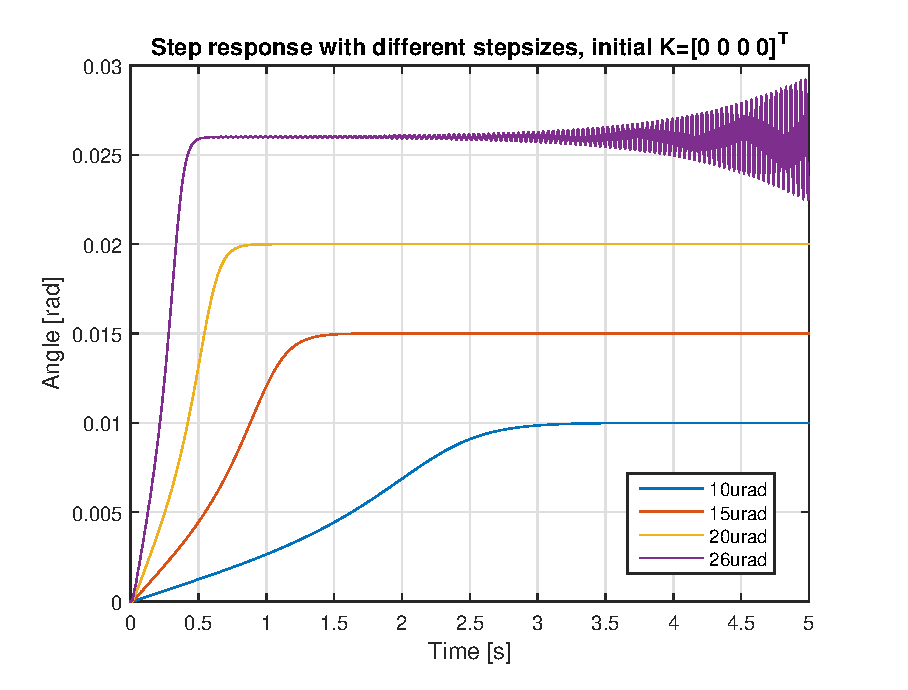
\includegraphics[width=0.7\textwidth]{fig/matlab/stepresponse.eps}
  \caption{\label{fig:step_adaptive} Step responses to stepsizes of 10, 15, 20 and 26 mrad.}
\end{figure}

\begin{figure}[h!]
  \centering
  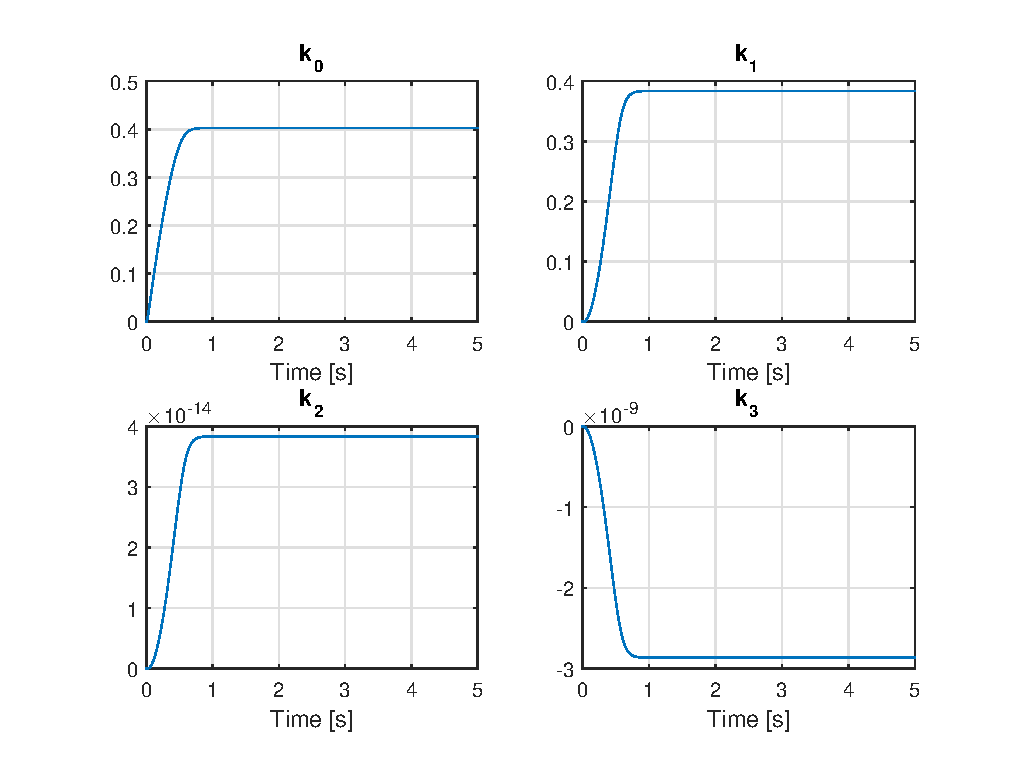
\includegraphics[width=0.7\textwidth]{fig/matlab/k.eps}
  \caption{\label{fig:hysteresis} Adaptation process of control parameters $k_i$ with a 20 mrad step.}
\end{figure}


\begin{figure}[h!]
  \centering
  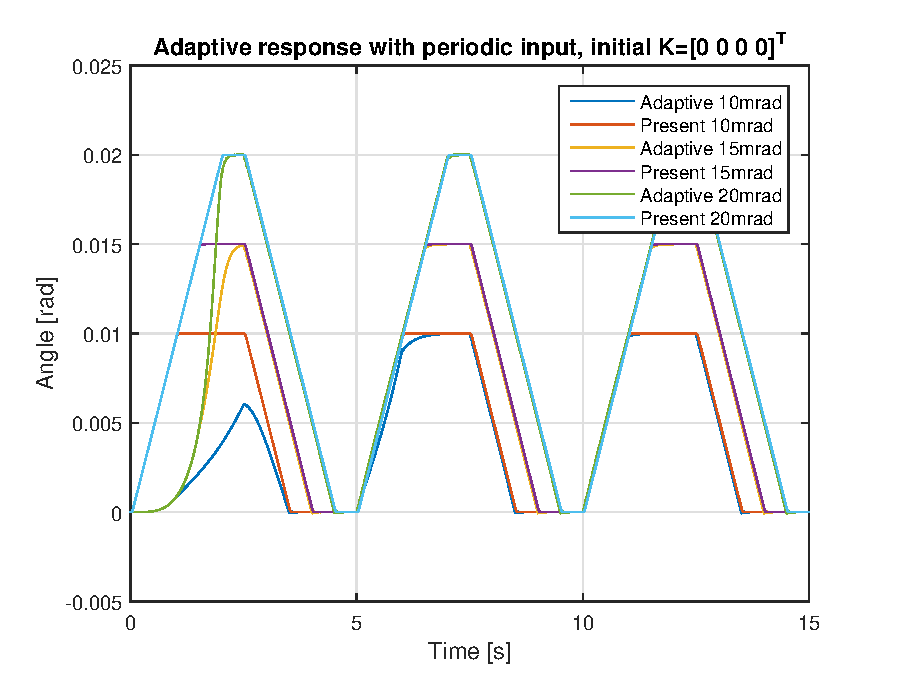
\includegraphics[width=0.7\textwidth]{fig/matlab/periodicresponse.eps}
  \caption{\label{fig:periodic_resp}Illustration of the hysteresis effect.}
\end{figure}

\begin{figure}[h!]
  \centering
  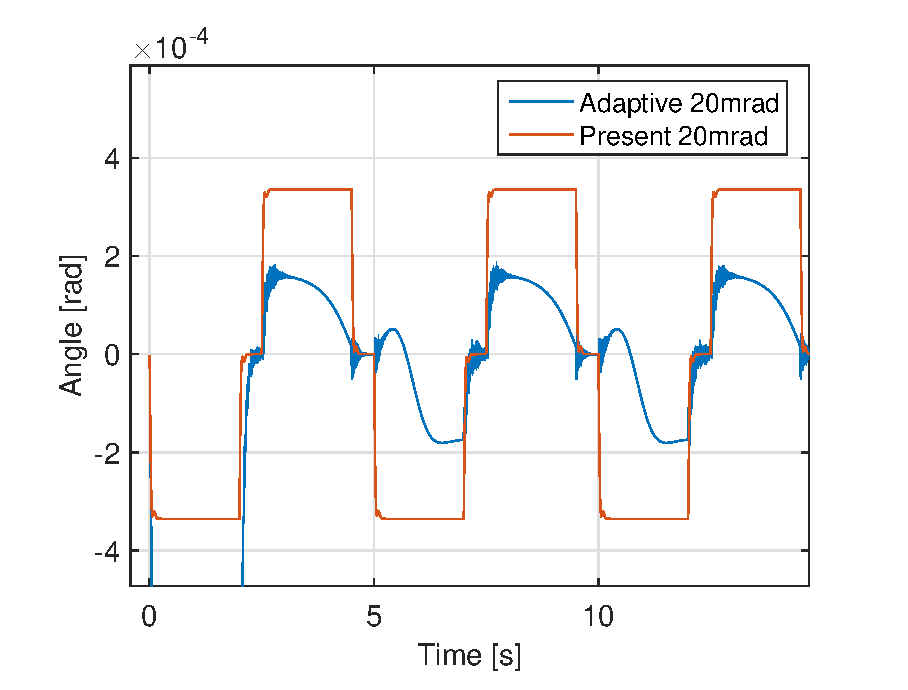
\includegraphics[width=0.7\textwidth]{fig/matlab/trackingerror.eps}
  \caption{\label{fig:hysteresis}Illustration of the hysteresis effect.}
\end{figure}

\begin{figure}[h!]
  \centering
  \includegraphics[width=0.7\textwidth]{fig/matlab/driftofmodelparameterover05s.eps}
  \caption{\label{fig:hysteresis}Illustration of the hysteresis effect.}
\end{figure}

\begin{figure}[h!]
  \centering %crop: left bottom right top
  \subfloat[][\label{fig:dist}Step response]{
  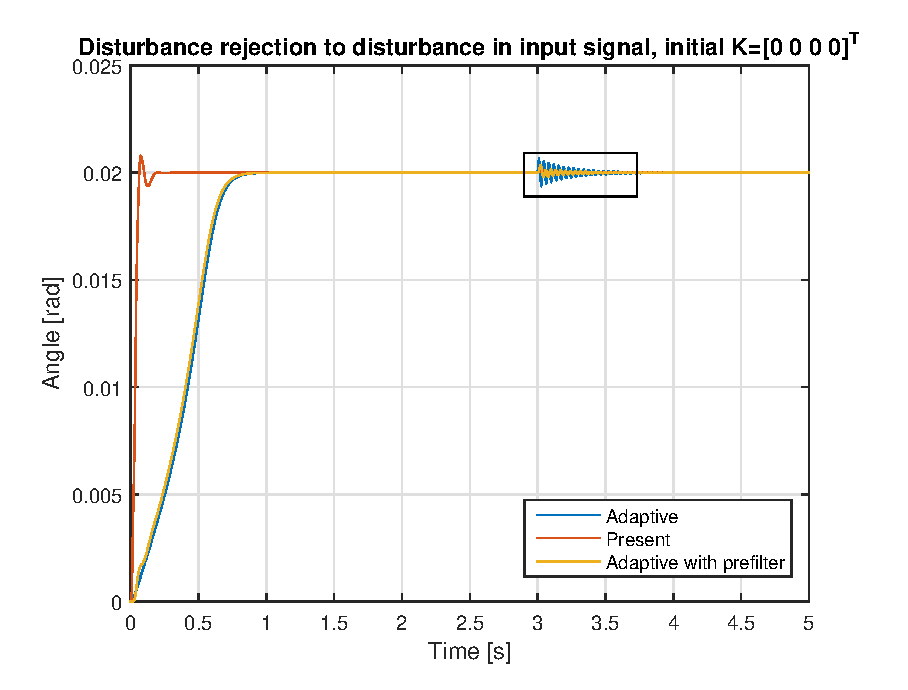
\includegraphics[width=0.45\textwidth]{fig/matlab/distrejection.eps}}
  \qquad
  \subfloat[][\label{fig:distzoom}Zoom in on disturbance]{
  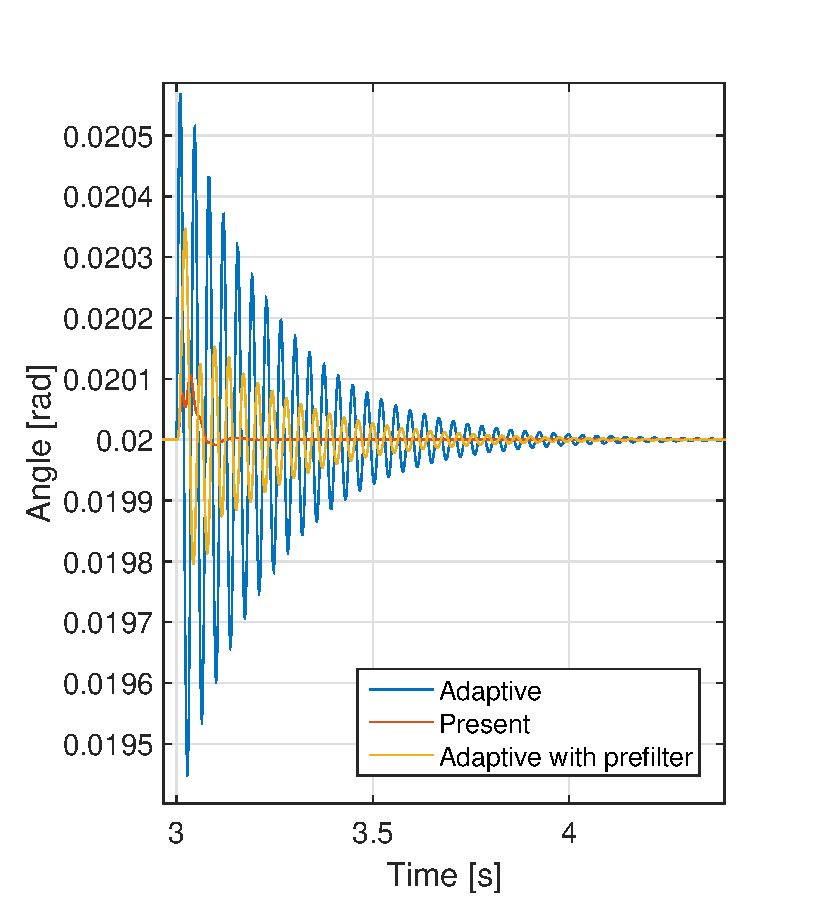
\includegraphics[width=0.45\textwidth]{fig/matlab/distrejection_zoom.eps}}
  \caption{\label{fig:distrejection} Shows how well the controller attenuates a disturbance glitch (amplitude of $5.1 \times 10^{-3}$) added to the input signal at $t=3s$. The whole step response is shown in (a) while a zoom in on the boxed area in (a) is presented in (b).}
\end{figure}

\begin{figure}[h]
  \centering %crop: left bottom right top
  \subfloat[][\label{fig:dist}Step response]{
  \includegraphics[width=0.45\textwidth]{fig/matlab/modelerror.eps}}
  \qquad
  \subfloat[][\label{fig:distzoom}Bode plot of perturbed model]{
  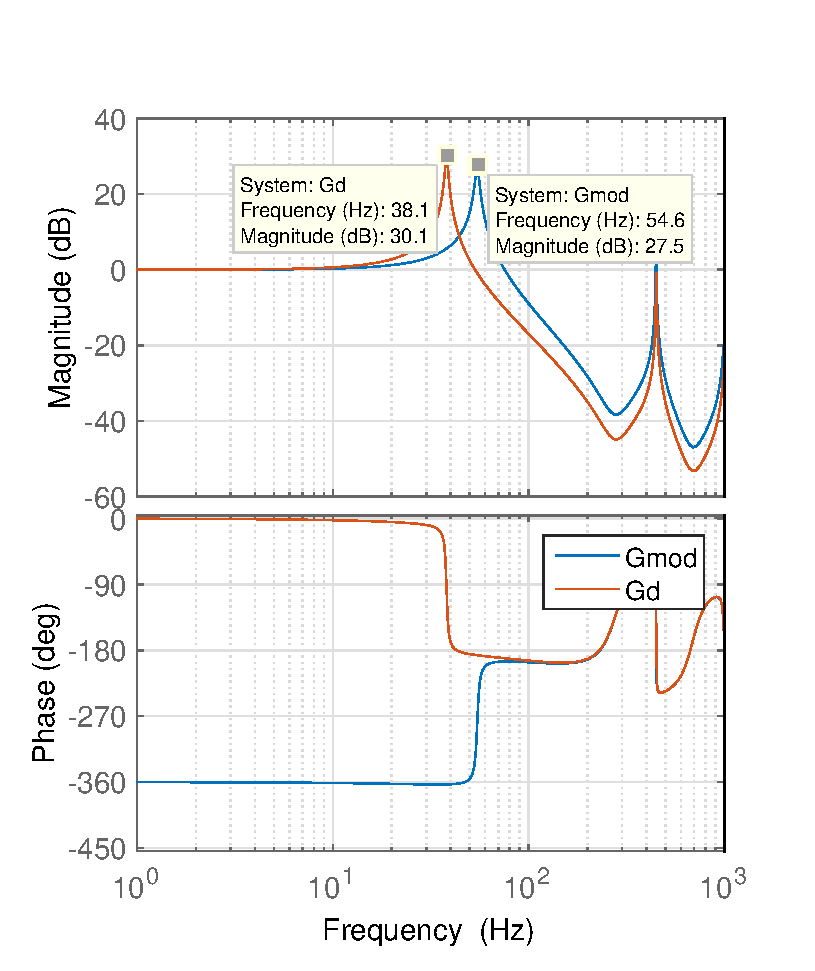
\includegraphics[width=0.47\textwidth]{fig/matlab/bode_modelerror_pole.eps}}
  \caption{\label{fig:distrejection} Shows how well the controller attenuates a disturbance glitch (amplitude of $5.1 \times 10^{-3}$) added to the input signal at $t=3s$. The whole step response is shown in (a) while a zoom in on the boxed area in (a) is presented in (b).}
\end{figure}


\section{Experimental Results}
\subsection{Setup}
The experiments have been conducted on the considered rotational stage described in Section~\ref{sec:rotational_stage}. A National Instruments PXI communicates with the Collimator and the rotaional stage, responsible for acquisition and control. To drive the rotaional stage it outputs a voltage between [-1, 7.5] V, this is amplified by a linear amplifier with a gain of \unit{20}{\volt/\volt} resulting in a [-20, 150] V signal input on the rotaional stage. The yaw angle, measured by the interferometric system is converted and sent to the PXI. The control loop is running at \unit{2}{\kilo\hertz}.
